\subsection{IoT Stream Processing Applications}
This tutorial analyzed IoT applications from two domains: sports and entertainment in addition to Industry 4.0. The application examples are based on commercial deployments using AGT International's\footnote{\url{http://www.agtinternational.com}} Internet of Things Analytics (IoTA) platform.

\iffalse
In sports and entertainment we described specific characteristics of IoT streaming applications and the associated challenge of choosing an appropriate streaming infrastructure. In the Industry 4.0 domain we showed how stream processing applications can be benchmarked using the HOBBIT benchmarking platform.
\fi

\para{Sports and Entertainment}
The example applications of this domain provide real-time narratives about highlights that are happening during a live event. This way, it is not necessary to watch the whole event, but one can be notified in real-time about such highlights based on insights derived from sensor data. For instance, in \emph{basketball}, sensors that have been successfully used in commercial deployments\footnote{\url{https://t.co/ZkQjQwXw13}} include smart shirts worn by players, microphones deployed to monitor the audience,  cameras and wristbands. Data from these sensors in combination with play-by-play data can be used to recognize behaviour, emotions, activities, actions, pressure and other physical aspects about the game. These insights are related to players, teams, fans and family that are preferably provided as semantic data streams. Semantic data access decouples applications from data providers and enables domain experts to better work with the data, e.g. for generating content and distributing it via social media.
%Figure Basketball ?

Another example is \emph{mixed martial arts}\footnote{\url{https://youtu.be/vataVq9gY_o}} in which sensors such as cameras, smart floors and a sensor embedded in a fighter's glove\footnote{\url{http://bit.ly/2D4lCqD}} are used in order to determine a range of insights including punch strength and stress levels of each fighter (Figure~\ref{FIG:FightStreams}). In this example, it is important that insights can be delivered in real-time without noticeable delay compared to a broadcast of the fight.

\begin{figure}[t]
\centering
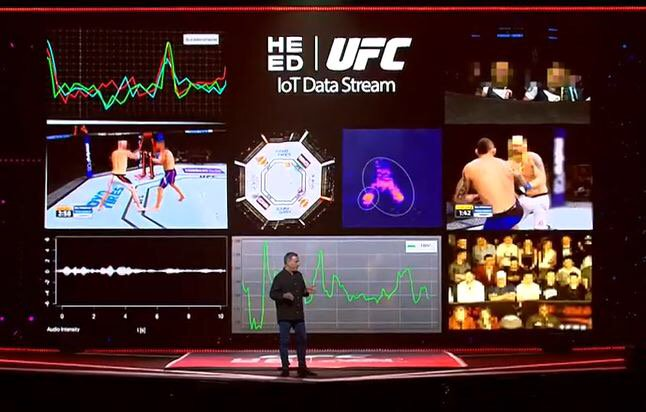
\includegraphics[scale=0.142]{pictures/DP6L8S9XkAYFMCw.jpg}
\captionof{figure}{A sample of IoT data streams that can be obtained during a fight.}
\label{FIG:FightStreams}
\end{figure}

In \emph{professional bull riding}, sensors are attached to riders and bulls and used in order to quantify the bull's and rider's performance\footnote{\url{http://bit.ly/2CXpc2g}}. As this information is among others used for automatic scoring, it is of particular importance that analytic results are available as soon as the ride is finished. Similarly, a range of wearable sensors are used for creating event highlights for participants at \emph{mass sport events} such as the Color Run\footnote{\url{https://thecolorrun.com/}}. In the \textsf{CPaas.io} project\footnote{\url{http://www.cpaas.io}}, an application has been developed to use action cameras and fitness bands to automatically detect event highlights based on the the runner's activity, emotions, dance energy levels, and many more metrics. In this application, real-time aspects include scenarios in which event highlights are being directly sent to friends of the participants.

\para{Industry 4.0}
For this domain, the tutorial presented applications related to \emph{predicting energy peaks} and \emph{predictive maintenance}. In principle, predicting energy peaks can help in reducing energy costs as electricity bills of industrial consumers contain a pricing component that incurs higher charges for higher peaks of electrical load. For a small to medium enterprise, avoiding such peak load events can lead to significant savings~\cite{strohbach_and_toll_2016}. This can be achieved by predicting expected peaks e.g. up to 30 minutes ahead of time and taking precautious measures such as temporarily switching off high energy consumers such as air conditioning.

For \emph{predictive maintenance}, the tutorial presented an application for detecting anomalous machine states in order to reduce maintenance costs. For instance, in injection molding machines a sudden high energy consumption may indicate that an injection nozzle is jammed and checking the machine may avoid further damage. The tutorial reported about the DEBS Grand Challenge 2017~\cite{gulisano_et_al_2017} that has been designed to objectively measure some of these requirements using pre-defined machine learning algorithms and RDF streaming data. The main KPI for the challenge was latency. The original data set has been provided by \textsf{Weidmüller}\footnote{\url{http://www.weidmueller.de}}. For reasons of confidentiality, the organizers provided a mimicked data set\footnote{\url{https://hobbit.iminds.be/dataset/weidmuller}}. The systems under test were evaluated using the \textsf{HOBBIT} benchmarking platform\footnote{\url{http://bit.ly/2muMNkY}} that ensured the objectivity of quantifying the performance of distributed stream processing pipelines. \iffalse As we used a pre-defined algorithm for detecting anomalies, we expected full correctness from all systems and compared latency and also measured throughput.\fi Overall, 7 out of 14 participating teams in the challenge passed the correctness test. The fastest system~\cite{amariei_et_al_2017} achieved an average latency of about 39ms. The DEBS Grand Challenge 2017 benchmark is openly available as part of the HOBBIT platform.

%Systems under test had to correctly answer a pre-defined query that describes an anomaly in the expected machine states. The task involved to find k cluster centers in a sliding window in order to identify the machine states. As a next step, it was required to build a Markov model over the sliding window and use it to determine the probability of the last N state transitions. Finally, if the probability is below a given threshold the system under test had to report an anomaly. Machines could dynamically leave and join.




%\subsubsection{Choosing the Streaming Infrastructure}
%When choosing a streaming infrastructure fulfilling the requirements of the above application scenarios, we face the following challenges

%\begin{itemize}
%  \item Lack of standardized query language for streaming applications
 % \item Flexibility for Programming Languages
 % \item Low Latencies and short-lived stream processing pipelines
% semantic mapping has been briefly mentioned in the sports and entertainment app
%  \item Semantic mapping
%\end{itemize}

%While in the database world there are standardized query languages such as SQL and SPARQL, there is still no standard stream processing language (see Section \ref{sec:tut_lang}). As a consequence streaming applications are very closely coupled to the underlying stream processing system making the choice of the infrastructure a critical one.

%When considering the applications above, it becomes apparent that the implementation of a variety of analytical modules are required. However, there is a discrepancy between the tools and programming languages typically used by data scientist (Python, Julia, C/C++, R, Matlab, etc.) and the mainly JVM based languages (Java and Scala) that are supported in common stream systems as described in section \ref{sec:tut_systems}. Although python is increasingly supported in these systems, resource management of JVM external languages is badly supported. However, such external resources may be considerable, e.g. if machine learning models are involved. And languages other than Python are not directly supported at all.

%Finally, IoT streaming applications as described above require low latency processing pipelines rather than supporting an extremely high number of throughput. In addition there may be a large number of short-lived rather than a few long-lived processing pipelines. In typical settings there may thousands of sensor streams connected to the system and a multitude of analytical results created from all the streams. However, not all streams are equally important at all times. For instance, in a sports tournament there may be a couple of standard pipelines being set up for the duration of the tournament, but many more smaller pipelines are set up for the duration of a single match, half or quarter. Some pipelines are only set up, based on ad-hoc queries. For the shorter-lived pipelines it is extremely important that the pipeline including its analytics module can be set up extremely fast, i.e. below one second, including tasks such as the deployment and resource allocation of analytics module and the models they use. To our knowledge virtually all existing and mature frameworks focus on high throughput and long lived processing pipelines and thus do not fully support these requirements.

